\section{Flux Balance Analysis}
The genome-scale integrated networks are necessary tools used by metabolic engineers on model generation, theoretical and computational analysis for microbial organisms. In addition, the network theory tools expand the feasible space for the following analysis techniques in the field. 

\textcolor{red}{Introducing stoic. matrix. Explain how the two graphs are formally obtained by manipulated the stoichiometric matrix, explain the metabolite-centric network is $S*S^{T}$ and binarized. In contrast, the reaction-centric network is $S^{T}*S$ and binarized. Introduce the general idea of FBA as an optimization scheme in a steady-state solution space.}
Although the networks shown in Fig.~\ref{figure-metabolic-networks} do not contain any information about directionality or effectiveness of the reactions to the system, the set of rules take place in networks can be represented in more detail and stoichiometrically by an m-by-r matrix formulation (the so-called Stoichiometric Matrix $S$), whereas its column elements represent reactions that play a role in the chemical transformation, and its row elements represent metabolites as
\begin{equation} \tag{1}
	S =  \begin{bmatrix} 
		s_{11} & s_{12} & \dots  & s_{1r}\\
		s_{21} & s_{22} & \dots  & s_{2r}\\
		\vdots & \vdots &\ddots & \vdots \\
		s_{m1} & s_{m2} & \dots & s_{mr} 
	\end{bmatrix}=(s_{ij})\in \mathbb{Z}^{mxr},
	\label{stoichio}
\end{equation}

Fig.~\ref{figure-metabolic-networks} shows two differently constructed networks showing interactions between metabolites, intermediate or end products and metabolic reactions for a particular metabolism: Homo Sapien. In Fig.~\ref{figure-metabolic-centric} the graph nodes stand for the metabolites, graph edges are the reactions. In contrast, in Fig.~\ref{figure-reaction-centric} the roles are reversed so that the graph edges represent the metabolites, and the graph nodes represent the reactions.

\begin{figure}[!ht]
	\centering
	\begin{subfigure}{0.5\textwidth}
		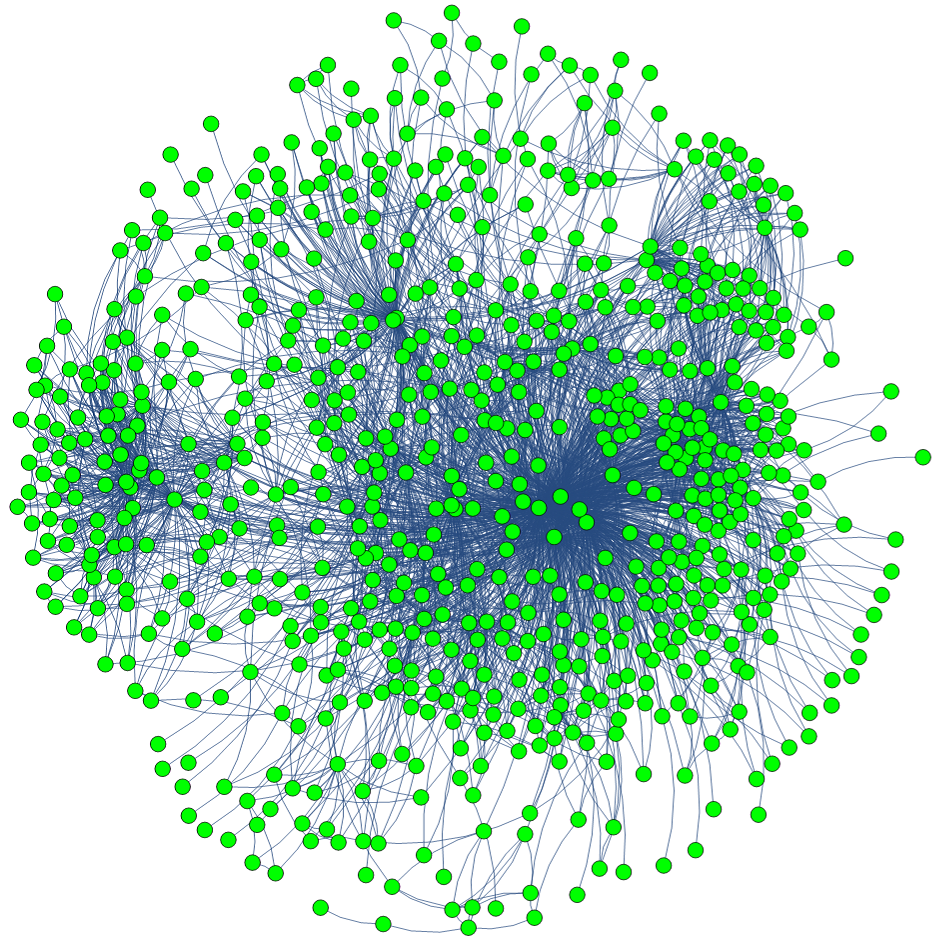
\includegraphics[width=1\linewidth]{../images/methodology-ORmodel-metabolic_centric_network.png}
		\caption{Metabolic-centric Network}
		\label{figure-metabolic-centric}
	\end{subfigure}\hfill% or \hspace{5mm} or  \hspace{0.3\textwidth}
	\begin{subfigure}{0.5\textwidth}
		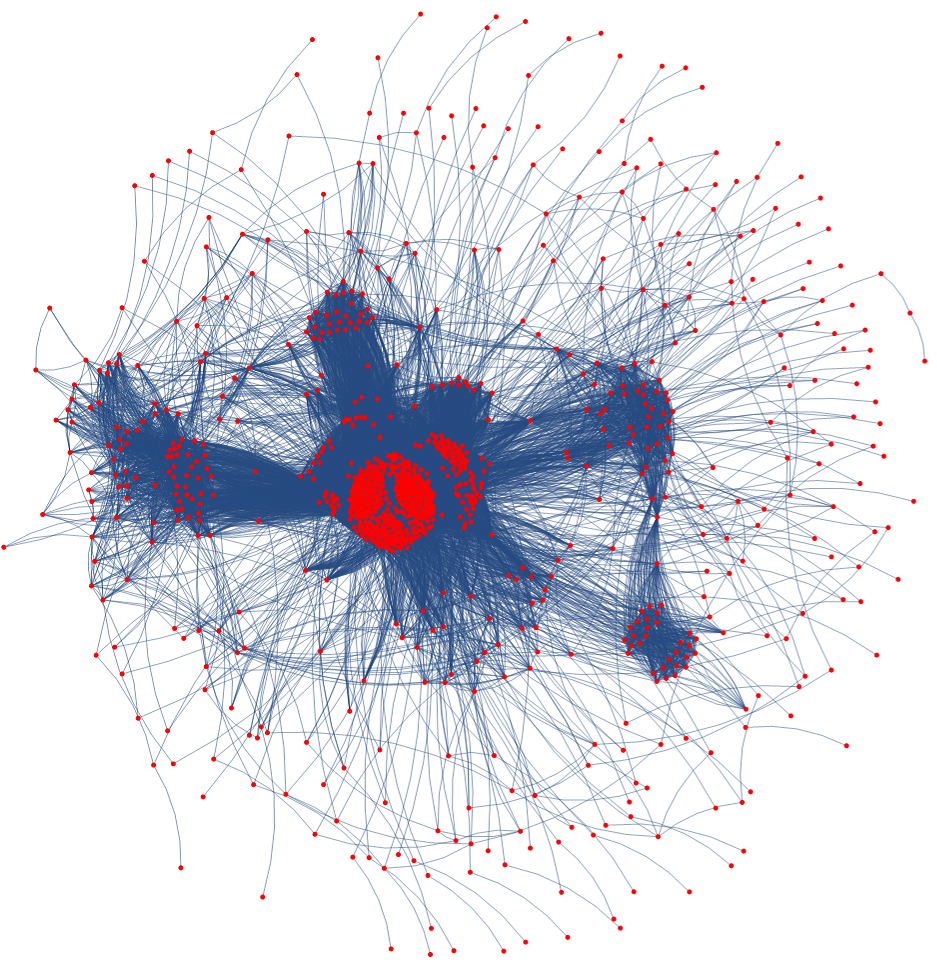
\includegraphics[width=1\linewidth]{../images/methodology-ORmodel-reaction_centric_network.png}
		\caption{Reaction-centric Network}
		\label{figure-reaction-centric}
	\end{subfigure}
	\caption{Network Representations for Homo Sapiens Metabolic Model}
	\label{figure-metabolic-networks}
\end{figure}

Studying biological metabolic systems, generated models to achieve cellular objectives like cell growth or ATP production brings the necessity of various tools to analyze reconstructed genome-scale networks.~\cite{KIM, HAO}. One of the commonly used tools is Flux Balance Analysis (FBA). It is a constraint-based modelling approach to simulate microbial metabolisms and can be applied to biochemical-reaction networks containing the chemical transformations and flux exchanges in that particular network~\cite{KAUFFMAN2003491, PRICE2004}.

while one can express the fluxes in a one-dimensional array (the so-called Flux Vector $V$) as 
\begin{equation} \tag{2}
	V = \begin{bmatrix}
		v_{1} \\
		v_{2} \\
		\vdots \\
		v_{r}
	\end{bmatrix}=(v_{i})\in \mathbb{R}.
	\label{solutionvector}
\end{equation}
$V$ contains flux exchange values for the corresponding reactions in the system and gives information about the flux distribution; hence, those can be both positive and negative real numbers. Definition of a mass balance ($S.V=0$) constraint in the FBA enables us to analyze the metabolic network operations in a steady-state~\cite{KAUFFMAN2003491,PRICE2004}.
%(resulting steady state vectors/resulting optimized solution vectors)
\begin{equation} \tag{3}
	S.V = \begin{bmatrix} 
		s_{11}v_{1} + s_{12}v_{2} + \dots + s_{1r}v_{r} \\
		s_{21}v_{1} + s_{22}v_{2} + \dots + s_{2r}v_{r} \\
		\vdots \\
		s_{m1}v_{1} + s_{m2}v_{2} + \dots + s_{mr}v_{r} 
	\end{bmatrix}=
	\begin{bmatrix} 
		0 \\
		0 \\
		\vdots \\
		0
	\end{bmatrix}.
	\label{massbalanceconstraint}
\end{equation}
The higher amount of metabolite consideration in the set of rules, $S$, in other words, the larger matrix size by its rows amount means the more complex organization structure taken into account while preserving the steady-state in the whole system.

More than one steady-state solution might be present since it is impossible to identify all constraints in a cellular system~\cite{KAUFFMAN2003491}. Therefore, one can formulate an optimization approach to identify reaction network steady-states that maximize the biomass~\cite{KAUFFMAN2003491,PRICE2004} or control the production of specific metabolites~\cite{VARMA1993} within a defined objective function under the consideration of the system constraints. According to Price et al. (2004),
there are three primary purposes to generate objective functions: to discover allowable characteristic properties in the genome-scale network reconstruction; to mimic probable physiological functions like biomass or ATP production to be able to determine likely physiological states; and lastly, to design a genetic variant or sub-type to obtain a desired particular product~\cite{PRICE2004}.

The objective function can be thought as a production plan that gives an idea about the diversity of products that the relevant system can produce, and one can express its coefficients in a one-dimensional array as
\begin{equation} \tag{4}
	O =  \begin{bmatrix}
		o_{1} & o_{2} & \dots  & o_{r}\\
	\end{bmatrix}=(o_{i})\in \mathbb{R}.
	\label{objectivecoefficients}
\end{equation}
As given in Eq.\eqref{biomassmaximisation}, the Objective Function, $Z$, rules the maximized output based on its non-zero coefficients, which are the decisive ones for the flux elements of $V$ to be considered.
\begin{equation} \tag{5}
	Z = O.V = (o_{1}v_{1} + o_{2}v_{2} + \dots + o_{r}v_{r})\in \mathbb{R}_{\ge0}.
	\label{biomassmaximisation}
\end{equation}
Stoichiometry and mass-balance are the constraints introduced so far in Eq.\eqref{stoichio} and Eq.\eqref{massbalanceconstraint}. In addition, upper and lower bounds are introduced for particular fluxes in $V$ during the optimization process. The bounds are used in the reactions for uptake and secretion of any organic metabolite. In the uptake reactions, nutrients are transported to the inside of the metabolic network. In the secretion reactions, products are exported to the outside of the network. The rest of the fluxes in $V$ are used in the exchange reactions, namely the intermediate reactions in the network. The constraints are decisive on the reactions for uptake and secretion, whereas no limitation is considered in the exchange reactions. Quantification of imported nutrients and exported outputs (the so-called Resources and Wastes) by constraining them with upper and lower bounds to fulfil a single objective function goal might play a significant role in the optimization process.

 \begin{figure}[!ht]
	\begin{center}
		\makebox[\textwidth]{
			\centering
			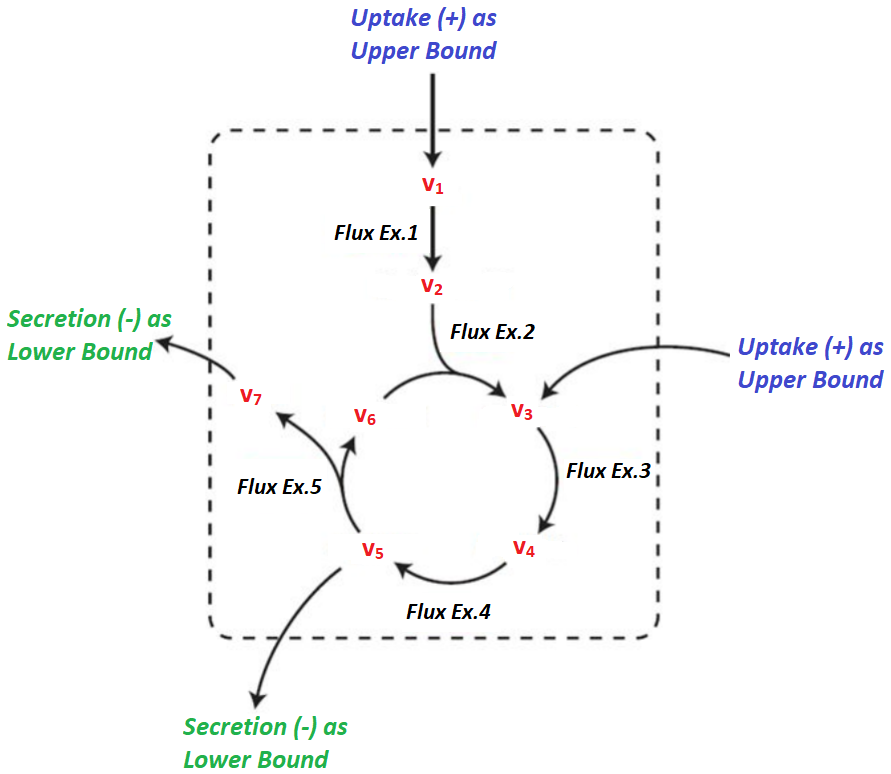
\includegraphics[width=0.57\linewidth]{../images/methodology-ORmodel-uptake_secretion_cartoon.png}}
		\caption{A Simplified Reaction-centric Network Sketch Shows The Reactions for Exchange, Uptake and Secretion.}
		\label{figure-uptake-secretion-cartoon}
	\end{center}
\end{figure}

The above-explained optimization process is a linear programming problem since the mass balance (Eq.\eqref{massbalanceconstraint}), the Objective Function (Eq.\eqref{biomassmaximisation}), and linear equations formulate the upper \& lower bounds for fluxes. The linear optimization result maximizes the structured Objective Function in the form of a flux distribution~\cite{KAUFFMAN2003491,PRICE2004}. Since each term in Eq.\eqref{biomassmaximisation} is a produced biomass expression for the fluxes, the summation of those terms will give the overall growth of the system for a single network state.

\subsection*{Fluxes for Uptake and Secrete Reactions}
\addcontentsline{toc}{subsection}{Fluxes for Uptake and Secrete Reactions}%
Let
\begin{equation} \tag{7}
	V^{*}=(v^{*}_{1}, v^{*}_{2},\dots, v^{*}_{x})= (a_{i}\le v^{*}_{i}\le b_{i})\in V
	\label{constrainedfluxlist}
\end{equation}
is a set of fluxes picked from $V$ to be limited with the bounds: $a_{i}$ and $b_{i}$ which are used in the reactions for uptake and secretion as previously introduced.
\subsection*{Upper and Lower Bounds}
\addcontentsline{toc}{subsection}{Upper and Lower Bounds}%
\subsection*{Objective Functions}
\addcontentsline{toc}{subsection}{Objective Functions}%